\subsection{Introduction}
Spike Sorting can be defined as the grouping of spikes into clusters
according to the similarity of their shapes.\\
This is useful only if the following assumption is made: each neuron tends
to fire spikes with a peculiar (distinguishable) extracellular shape.
As a consequence, it is possible to determine the activity of each one of these
neurons according to the measured spikes associated with it through Spike Sorting.\\
There are 3 reasons making Spike Sorting useful:
\begin{itemize}
    \item Increase the scale: as modern devices (MEAs) record from large populations
          of neurons at the same time, it is desirable to derive the inidividual
          activity of as many neurons as possible.
    \item Carry out new types of analysis: it might be interesting to study
          connectivity patterns of close-by neurons or perform analysis at
          single-neuron level.
    \item Have acess to sparsely firing neurons: it is desirable to understand
          the typical patterns of a specific kind of neuron, allowing to study its
          specific function.
\end{itemize}
Despite everything, Spike Sorting still present a number of major problems:
\begin{itemize}
    \item Dealing with background noise.
    \item Neurons in the same area might emit spikes with a similar shape (there
          is no way to perfectly know which neuron fired apart from imaging techniques).
    \item Neurons in the same area might emit spikes with a smaller amplitude.
    \item Background activity of distant neurons pollute the recorded signal.
    \item Waveform misalignment.
    \item Variation of the spike shape as a function of recent firing history
          (not time-invariant shape).
\end{itemize}
In the following an image of the whole Data Recording, Spike Detection, and
Spike Sorting process:
\begin{figure}[H]
    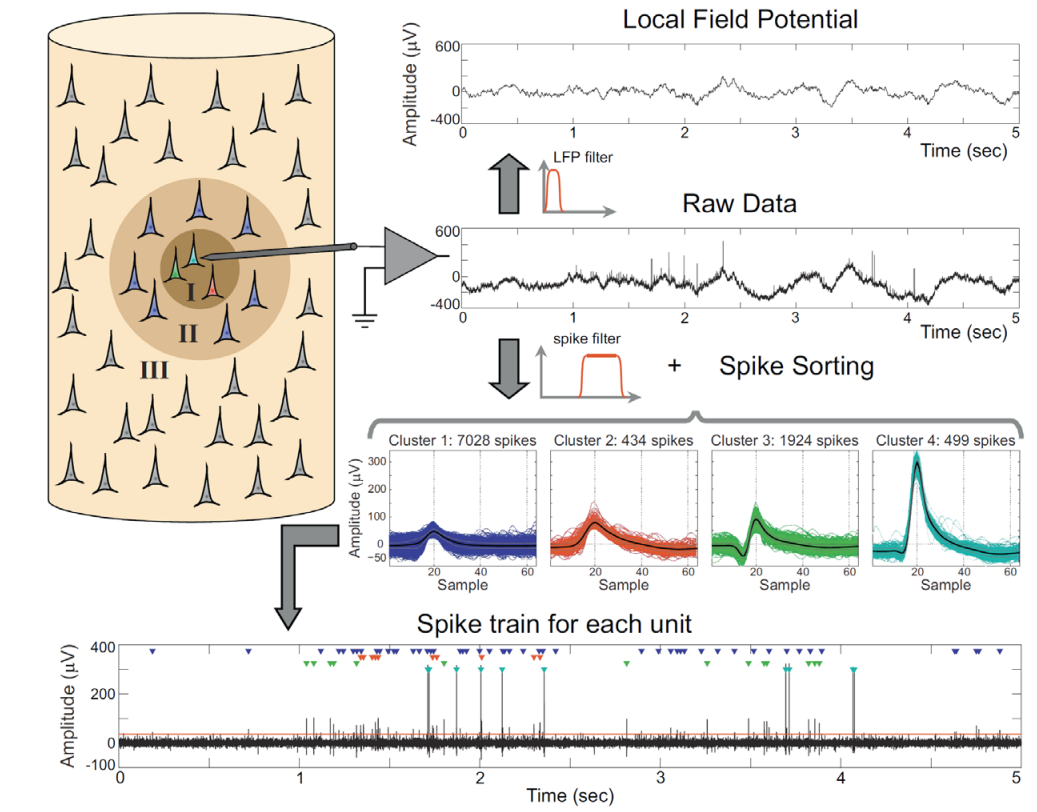
\includegraphics[scale=0.45]{3_1}
    \centering
\end{figure}


\subsection{Spike Sorting methods}
When it comes at Spike Sorting, there are 3 main approaches:
\begin{itemize}
    \item \textbf{Amplitude discriminator:} separate spikes according to their amplitude.
          This method does not take into account the shape of a spike, only its
          amplitude.
    \item \textbf{Template matching:} select a characteristic spike shape for each cluster
          and divide the spikes among the clusters via matching with the templates,
          according to an appropriate distance measure. The main issues of this
          approach is that the templates might need to adjust during the experiment
          and that it is necessary a good way to select the templates.
    \item \textbf{Window discriminator:} assign spikes crossing one or more windows
          to the same neurons. Also in this case issue may arise, especially spike
          shapes might overlap.
\end{itemize}
Please note that these algorithms perform Spike Detection and Spike Sorting at the same time.
In general, Spike Sorting is carried out by following the steps shown below:
\begin{figure}[H]
    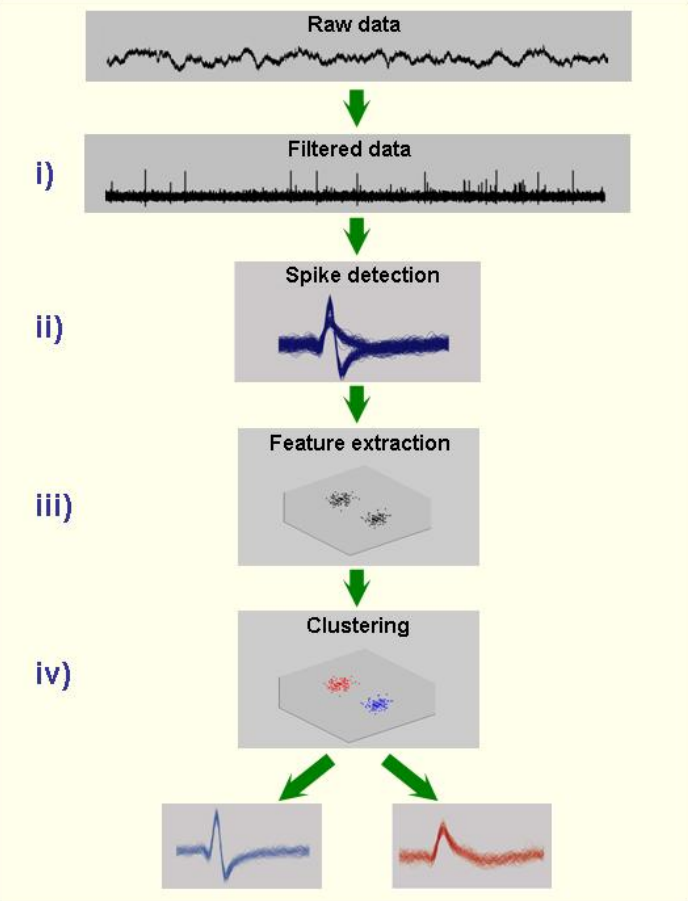
\includegraphics[scale=0.5]{3_2}
    \centering
\end{figure}
\subsubsection{Filtering}
The first step consists in filtering out the low frequency components
(\(<\) 300 Hz), in particular the local field potentials, in order to visualize
spikes.
To do so, a band 300-3000 Hz band-pass filter is employed: all the
frequencies outside the specified range are rejected.
\subsubsection{Spike Detection}
Spikes are commonly detect by using an amplitude threshold, as seen in the
previous chapter. The optimal threshold can be set manually or automatically
computed as a multiple of the standard deviation (SD) of the signal, where
\begin{align*}
    SD=\sigma=median\biggl(\frac{|x|}{0.6745}\biggr)
\end{align*}
\subsubsection{Feature Extraction}
Let's set the number of observations (i.e. spikes) to \(n\) and the
variables (data points) to \(m\), thus a \(m\)-dimensional space is obtained.
The idea is to extract a number of features \(p\), such that it has a lower
dimensionality (\(p<m\)).\\
The \(p\)-dimensional features can be selected in different ways:
\begin{itemize}
    \item Take basic properties of the spikes (amplitude, width, energy, ...),
          not optimal in differentiating spikes.
    \item Select a low number of components from a dimensionality reduction
          technique, such as PCA. Notice that these components represent the directions
          of maximum variance of the data, not necessarily the best separation.
    \item Use wavelets, obtaining a time-frequency decomposition of the signal
          with optimal resolution in both time and frequency domains.
\end{itemize}
\paragraph{Principal Component Analysis (PCA)}
It is an unsupervised dimensionality reduction technique, which can be used
also for feature extraction purposes. Data are rotated according to a new space
having the orthogonal axes in the directions of maximum variance, then the new
obtained principal components are ordered by their contribution to the overall
variance, allowing to select only a fraction of the total number of components,
still approximating the original data fairly well. Low variance is often
interpreted as noise.
\paragraph{Wavelets}
The wavelet transformation (WT) is a time-frequency representation of the signal,
similar to the Fourier transform, but breaking the signal into its wavelets.
It may be defined as the convolution between the signal \(x(t)\) and the
wavelet functions \(\psi_{a,b}(t)\):
\begin{align*}
    W_\psi X(a,b)=\left\langle x(t)|\psi_{a,b}(t) \right\rangle
    \quad\quad\quad\quad\text{with}\quad
    \psi_{a,b}(t)=|a|^{-\frac{1}{2}}\psi\biggl(\frac{t-b}{a}\biggr)
\end{align*}
where \(a\) and \(b\) are scale and translation parameters.\\
Contracted wavelet function matches the high-frequency components, while
dilated wavelet matches the low-frequency components, thus details of the signal
at several scales can be obtained.\\
The wavelet method coefficients are then selected such that they allow to
distinguish well the spike shapes, in particular multi-modal distributions
are preferred and unimodal distributions are to be avoided.
\subsubsection{Clustering}
The final step of spike sorting is to group spikes with similar features into
clusters, corresponding to different neurons. Different approaches are available:
\begin{itemize}
    \item Manual clustering
    \item Bayesian classification
    \item Expectation-Maximization methods
    \item Hierarchical clustering
    \item K-Means
    \item Superparamagnetic clustering
\end{itemize}
\paragraph{Superparamagnetic Clustering}
This method is inspired by statistical mechanics, it does not assume
a-priori distributions for the data, and exploit only one parameter to
form clusters: temperature.\\
The \(p\)-selected features of a generic \(i\)-th spike are represented by a
point \(x_i\) in a \(p\)-dimensional phase space. Then, let's define the
interaction strength between two points \(x_i\) and \(x_j\):
\begin{align*}
    J_{ij}=
    \begin{cases}
        \begin{matrix}
            \frac{1}{K}\exp{\biggl(-\frac{\|x_i-x_j\|^2}{2a^2}\biggr)} &  & \text{if}\,x_i\,\text{is a nearest neighbor of}\,x_j \\
            0                                                          &  & \text{else}
        \end{matrix}
    \end{cases}
\end{align*}
where \(a\) is the average nearest-neighbor distance and \(K\) is the
number of nearest neighbors.
As a consequence, similar spikes will exhibit a strong interaction.\\
At this point, a random state is assigned to each point \(x_i\) and \(N\) Monte
Carlo iterations are run for different temperatures \(T\). A point \(x_i\) is
randomly selected and its state is randomly changed to \(s_{new}\).
The probability that the nearest neighbors of \(x_i\) will change their state
to \(s_{new}\) is given by:
\begin{align*}
    p_{ij}=1-\exp{\biggl(-\frac{J_{ij}}{T}\delta_{s_i,s_j}\biggr)}
\end{align*}
This implies that close points will change their status together,
forming clusters of spikes with similar shape.\\
In particular
\begin{itemize}
    \item High temperatures correspond to a low probability of
          changing the state \(\Rightarrow\) states change randomly, thus no clusters
          are formed (paramagnetic phase).
    \item Low temperatures correspond to a high probability of changing to the
          same state, regardless of the interaction strength \(J_{ij}\)
          \(\Rightarrow\) all states are changed to the same, thus all spikes belong
          to the same cluster (ferromagnetic phase).
    \item Medium temperatures correspond to a phase in which only similar spikes
          will change their state together, forming meaningful clusters
          (Superparamagnetic phase).
\end{itemize}


\subsection{Miscellaneous}
In the following are reported some further remarks and considerations concerning
Spike Sorting.
\subsubsection{Spike Sorting issues}
The main issues when it comes to Spike Sorting are listed below:
\begin{itemize}
    \item \textbf{Electrode Drift:} waveforms of a given neuron vary over
          time and may be assigned to multiple clusters.
    \item \textbf{Tetrodes:} tetrode recordings can be exploited to improve
          spike sorting results, since they allow the visualization of single
          neurons from different positions.
    \item \textbf{Overlapping Spikes:} this phenomenon can be observed when
          two close-by neurons fire in synchrony or with a small delay. Still
          an open issue in Spike Sorting.
    \item \textbf{Bursting Cells:} a burst is the firing of a fast sequence
          of spikes by a neuron. Successive spikes in a burst may have decreasing
          amplitude and may be mistakenly considered as separate clusters.
\end{itemize}
\subsubsection{KiloSort}
The aim is to develop a fully automated, scalable, and accurate spike sorter,
removing the burden of this task from researchers. It belongs to the template
matching class of Spike Sorting algorithms.
The main hypothesis of KiloSort is that spatial and temporal shapes of a waveform
provide all the information necessary to assign a given spike to a neuron.
This algorithm exploits template matching in both Spike Detection and Spike
Sorting, which are condensed into a single unified model describing the voltage
\(V\) of channel \(i\) at the time instant \(t\):
\begin{align*}
    V(i,t)=\sum_{k=1}^{N_{spike}}A_{\sigma(k)}(i,t-t_k)\cdot x(k) + noise
\end{align*}
with \(A_{\sigma(k)}(i,t-t_k)\) being the spike template for the \(k\)-th neuron
and \(x(k)\) the amplitude of the spike emitted by the \(k\)-th neuron.
\subsubsection{Performance evaluation}
Different Spike Sorting methods can be compared by testing them on simultaneous
extracellular and intra-cellular recordings datasets, in a similar fashion w.r.t.
Spike Detection. The same metrics are generally used. The SpikeForest project
aims at benchmarking and testing the finest and most recent Spike Sorting
algorithms.